\documentclass[a4paper,11pt]{article}

\usepackage{mlsubmit}

\begin{document}

\initmlsubmision{1}                              					% assignment number
								{Talla Aravind Reddy}      						           		% your name
								{14746}																		% your roll number

\begin{mlsolution}

\section*{Part 1}
Let $z=(x_1,y_1)$. We are given ${z_r}=(0,1)$ and ${z_g}=(1,0)$.
\\For the decision boundary, $d(z,z_r) = d(z,z_g)$ 
\\$\implies \langle z-z_r,U(z-z_r)\rangle = \langle z-z_g,U(z-z_g)\rangle $ 
where $U = \begin{bmatrix} 3 & 0  \\ 0 & 1 \end{bmatrix}$
\\$\implies 3x_1^2 + (y_1 - 1)^2 = 3(x_1 - 1)^2 + y_1^2 $
\\$\implies 3x_1^2 - 3(x_1 - 1)^2 =  y_1^2 - (y_1 - 1)^2$
\\$\implies 6x_1- 3 =  2y_1 - 1$
\\$\implies 3x_1 = y_1 + 1$
\\$\implies 3x = y+ 1$ is the decision boundary.

\section*{Part 2}
For the decision boundary, $d(z,z_r) = d(z,z_g)$ 
\\$\implies \langle z-z_r,U(z-z_r)\rangle = \langle z-z_g,U(z-z_g)\rangle $ 
where $U = \begin{bmatrix} 1 & 0  \\ 0 & 0 \end{bmatrix}$
\\$\implies x_1^2 = (x_1 - 1)^2$
\\$\implies 2x_1 - 1 =  0$
\\$\implies x_1 = \frac{1}{2}$
\\$\implies x = \frac{1}{2}$ is the decision boundary.

\begin{figure}[th]%
\centering
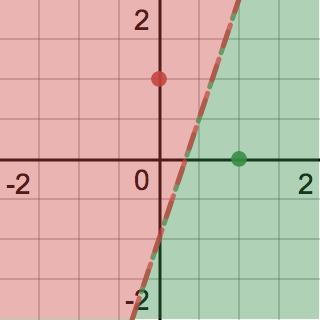
\includegraphics[width=0.3\columnwidth]{q1_graph1.png}%
\hfill
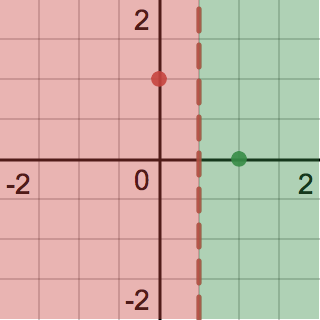
\includegraphics[width=0.3\columnwidth]{q1_graph2.png}%
\caption{The figure on the left shows the decision boundary for part 1 i.e $3x = y+ 1.$\newline The figure on the right shows the decision boundary for part 2 i.e $x = \frac{1}{2}$.}%
\label{fig:proto}%
\end{figure}

\end{mlsolution}

\begin{mlsolution}
One likelihood distribution which leads to $\mathbf{\hat{w}}_{cls}$ as the MAP estimate for the model is the gaussian distribution with mean as $\langle \mathbf{w,x}^i \rangle$ \[
\mathbb{P}[y|\mathbf{x}^i,w] = \mathcal{N}(\langle \mathbf{w,x}^i \rangle,\sigma^2) = \frac{1}{\sqrt{2\pi\sigma^2}} \text{exp}\bigg(-\frac{(y-\langle \mathbf{w,x}^i \rangle)^2}{2\sigma^2}\bigg)
\]
\\The prior distribution encapsulates the fact that $||\mathbf{w}||_2 \leq r$. This can be achieved by a uniform distribution over the $d$-dimensional ball with origin as centre and radius $r$.\[
\mathbb{P}[\mathbf{w}] = \mathcal{U}(\mathbf{0},r) = 
     \begin{cases}
       \cfrac{\Gamma(\frac{d}{2} + 1)}{\pi^{\frac{d}{2}} r^d} &\quad\text{if }||\mathbf{w}||_2 \leq r\\
       0 &\quad\text{if }||\mathbf{w}||_2 > r\\
     \end{cases}
\]

\end{mlsolution}

\begin{mlsolution}
The likelihood part of the estimate is same as the previous question, therefore one likelihood distribution is  the gaussian distribution with mean as $\langle \mathbf{w,x}^i \rangle$ \[
\mathbb{P}[y|\mathbf{x}^i,w] = \mathcal{N}(\langle \mathbf{w,x}^i \rangle,\sigma^2) = \frac{1}{\sqrt{2\pi\sigma^2}} \text{exp}\bigg(-\frac{(y-\langle \mathbf{w,x}^i \rangle)^2}{2\sigma^2}\bigg)
\]
For the prior, we can take a multivariate gaussian distribution with mean at $\mathbf{0}$\[
\mathbb{P}[\mathbf{w}] = \mathcal{N}(\mathbf{w};\mathbf{0},\Sigma) = \frac{1}{\sqrt{(2\pi)^d |\Sigma|}} \text{exp}\bigg(-\frac{1}{2}\mathbf{w}^T\Sigma^{-1}\mathbf{w}\bigg)
\]
Here $\Sigma = \sigma^2
\begin{bmatrix} 
\frac{1}{\alpha_1} & 0 & \dots & \dots & 0
\\ 0 & \frac{1}{\alpha_2} & 0 & \dots & 0
\\ \vdots & 0 & \ddots & 0\dots & 0
\\ \vdots & \vdots & \vdots & \frac{1}{\alpha_{d-1}} & 0
\\ 0 & 0 & 0 & 0 & \frac{1}{\alpha_d}
\end{bmatrix}$ i.e a diagonal matrix with it's $i$'th diagonal entry as $\frac{\sigma^2}{\alpha_i}$ where $\sigma^2$ is the variance of the likelihood distribution.\[
\text{log }\mathbb{P}[\mathbf{w|X,y}] = C -\frac{1}{2\sigma^2}\sum_{i=1}^{n}(y^i-\langle \mathbf{w,x}^i \rangle)^2 -\frac{1}{2\sigma^2}\sum_{j=1}^{d} \alpha_j \mathbf{w}_j^2 \]
\[ \implies \mathbf{\hat{w}}_{\text{MAP}} = \text{arg min} \sum_{i=1}^{n}(y^i-\langle \mathbf{w,x}^i \rangle)^2 + \sum_{j=1}^{d} \alpha_j \mathbf{w}_j^2   \]

\section*{Closed form expression:}
We need to minimise \[ \mathcal{L} =  \sum_{i=1}^{n}(y^i-\langle \mathbf{w,x}^i \rangle)^2 + \sum_{j=1}^{d} \alpha_j \mathbf{w}_j^2   \]
 \[ \mathcal{L} =  ||\mathbf{Xw - Y}||^2 + \sum_{j=1}^{d} \alpha_j \mathbf{w}_j^2   \]
 \[ \nabla_w \mathcal{L} = 2\mathbf{X}^T(\mathbf{Xw - Y}) + 2\mathbf{D_{\alpha}w} \text{ where } D_{\alpha} \text{ is the diagonal matrix with entries } \alpha_1,\alpha_2 \dots \alpha_d \]
 \[ \nabla_w \mathcal{L} = 2((\mathbf{X^T X + D_{\alpha})w} -\mathbf{X^T Y})\]
 \[\nabla_w \mathcal{L}= 0  \]
 \[ \iff (\mathbf{X^T X + D_{\alpha})w} -\mathbf{X^T Y} = 0 \]
 \[ \iff (\mathbf{X^T X + D_{\alpha})w}  = \mathbf{X^T Y} \]
 \[ \iff w = \mathbf{(X^T X + D_{\alpha})^{-1} X^T Y} \]
\end{mlsolution}

\begin{mlsolution}
 Lorem ipsum dolor sit amet, consectetur adipiscing elit. Duis feugiat vehicula dolor, sed ultricies leo. Phasellus euismod dictum felis in euismod. Proin pretium vel neque in placerat. Proin imperdiet egestas vulputate. Etiam faucibus accumsan ante non viverra. Duis ultrices ac odio vel sodales. In maximus gravida dolor, ut commodo lacus. Pellentesque ante massa, venenatis id aliquam et, posuere sed dui. Duis dignissim justo sit amet augue posuere fringilla. Suspendisse at nisi gravida, mattis justo sit amet, elementum elit. Praesent et massa ornare, consequat dui eget, ornare risus. Duis est nibh, sollicitudin nec mattis non, mattis in leo. Donec finibus justo sed massa sagittis, non fermentum nibh dictum. Pellentesque et congue purus. Donec porta pretium porttitor.

Morbi euismod risus eu tortor ornare malesuada. Nunc sed sollicitudin neque, efficitur rhoncus tellus. Cras malesuada augue arcu. Sed sem odio, tincidunt quis laoreet ac, facilisis ut nibh. Quisque gravida dolor at egestas aliquam. Aenean mollis massa sit amet enim mattis, vel fermentum tortor facilisis. Donec pellentesque est velit, vitae posuere lorem tristique ut. 
\end{mlsolution}
					
\end{document}